
\documentclass[11pt, a4paper, oneside, british]{article}


%%
%% Pakete & Formalia
%%
\usepackage[british]{babel} % neue deutsche Trennungsregeln, etc
\usepackage[hidelinks]{hyperref} % Hyperlinks ohne Umrandungen
\usepackage{setspace} % Abstände zwischen Absätzen
\usepackage[left=2cm, right=2cm, top=2cm, bottom=2cm]{geometry} % Seitenränder
\setstretch{1.5} % 1,5 Zeilenabstand
\usepackage{lipsum}  % Dummy-Texte
\usepackage{titlesec} % define size for section headings
\usepackage[nohyperlinks, printonlyused]{acronym} % Abkürzungen
%\usepackage[utf8]{inputenc} % korrekte Darstellung von Umlauten
\usepackage[T1]{fontenc} % enable hyphenation for languages with accented characters


	
\usepackage{color, colortbl}

%% Schriftarten und -größen
\usepackage{fontspec}
%\setmainfont{Arial} % Hauptfont Arial (lualatex oder xelatex benötigt)
\titleformat{\section}{\normalfont\fontsize{12pt}{1.5}\bfseries}{\thesection}{1em}{} % Überschriften 1pt größer
\titleformat{\subsection}{\normalfont\fontsize{12pt}{1.5}\bfseries}{\thesubsection}{1em}{} % Überschriften 1pt größer
\titleformat{\subsubsection}{\normalfont\fontsize{12pt}{1.5}\bfseries}{\thesubsubsection}{1em}{} % Überschriften 1pt größer
\def\UrlFont{\rm} % Print URLs not in Typewriter Font
\renewcommand{\footnotesize}{\fontsize{10pt}{1.5pt}\selectfont}

% automatischens Einrücken von Absätzen verhindern
\usepackage{changepage}
\setlength{\parindent}{0pt}
% 6pt Abstand nur zwischen Absätzen
\setlength{\parskip}{6pt}{}

% Leerseite ohne Seitennummer, nächste Seite rechts
\newcommand{\blankpage}{
 \clearpage{\pagestyle{empty}\cleardoublepage}
}

% Grafiken einbinden
\usepackage{graphicx}
% center images and tables
\makeatletter
\g@addto@macro\@floatboxreset\centering
\makeatother



\hypersetup{
 pdfauthor={Ivo Prahm},
 pdftitle={Paper Plane Rotations}, 
  pdfsubject={DLMCSPSE},
 pdfkeywords={DLMCSPSE, Project},
 pdfcreator={lualatex},
 pdfproducer={lualatex},
}

%%
%% Bibliographie & Sondereinstellungen
%%
\usepackage[babel]{csquotes}
\usepackage[backend=biber, style=apa, pagetracker, apamaxprtauth=20 ]{biblatex}

%%
%% Source Code Setup
%%
\usepackage{listings}
\usepackage{color}
\definecolor{dkgreen}{rgb}{0,0.6,0}
\definecolor{gray}{rgb}{0.5,0.5,0.5}
\definecolor{mauve}{rgb}{0.58,0,0.82}

\lstset{frame=tb,
  language=Java,
  aboveskip=3mm,
  belowskip=3mm,
  showstringspaces=false,
  columns=flexible,
  basicstyle={\small\ttfamily},
  numbers=none,
  numberstyle=\tiny\color{gray},
  keywordstyle=\color{blue},
  commentstyle=\color{dkgreen},
  stringstyle=\color{mauve},
  breaklines=true,
  breakatwhitespace=true,
  tabsize=3
}

\usepackage{xltabular}
\usepackage{fontspec}

\setmainfont{Asap}[
    Path=./AsapFontFiles/,
    Scale=0.9,
    Extension = .ttf,
    UprightFont=*-Regular,
    BoldFont=*-Bold,
    ItalicFont=*-Italic,
    BoldItalicFont=*-BoldItalic
    ]

\setmonofont{JetBrainsMono}[
    Path=./JetbrainsFontFiles/,
    Scale=0.75,
    Extension = .ttf,
    UprightFont=*-Regular,
    BoldFont=*-Bold,
    ItalicFont=*-Italic,
    BoldItalicFont=*-BoldItalic
    ]

\usepackage{csquotes}

\usepackage{tcolorbox}
    
\definecolor{babyblue}{rgb}{0.82, 0.96, 0.936} 
\definecolor{default}{rgb}{0.160, 0.164, 0.180}
\definecolor{lightgray}{rgb}{0.922, 0.922, 0.922} 
\definecolor{textgray}{rgb}{0.494, 0.505, 0.537} 
\definecolor{linegray}{rgb}{0.866, 0.870, 0.882} 
\definecolor{TAGgreen}{rgb}{0.729, 0.862, 0.501} 
\definecolor{TAGred}{rgb}{0.929, 0.623, 0.576} 
\definecolor{TAGgray}{rgb}{0.866, 0.882, 0.878} 
\definecolor{TAGyellow}{rgb}{0.933, 0.788, 0.388} 
\definecolor{TAGpurple}{rgb}{0.478, 0.282, 0.627} 
\definecolor{purpleT}{rgb}{0.478, 0.282, 0.627} 

\tcbset{on line, boxsep=1pt, left=3pt,right=3pt,top=2pt,bottom=1pt,colframe=TAGgreen, colback=TAGgreen}

\setlength\intextsep{0mm}

\newcolumntype{P}[1]{>{\centering\arraybackslash}p{#1}}
\newcolumntype{M}[1]{>{\centering\arraybackslash}m{#1}}
\renewcommand\tabularxcolumn[1]{m{#1}}

\makeatletter
\renewcommand*{\apablx@ifrevnameappcomma}{\@secondoftwo}
\makeatother

\DefineBibliographyExtras{ngerman}{%
  \renewcommand*{\finalandcomma}{}%
}



%% Bibliographie einbinden
\addbibresource{references.bib} % your bib file


%% ++++++++++++++++++++++++++++++++++++++++++
%% Dokument
%% ++++++++++++++++++++++++++++++++++++++++++
\begin{document}
\color{default}

\pagenumbering{Roman} % Uppercase Roman numerals
% \pagenumbering{gobble} % switch off page numbering
%% Titelseite
\def\usesf{}
\let\usesf\sffamily % diese Zeile auskommentieren für normalen TeX Font

\newsavebox{\Tutorin}
\savebox{\Tutorin}{<Name des Tutors>}


\setlength{\unitlength}{1pt}

\begin{titlepage}
%\vspace*{-39pt}\hspace*{300pt}\includegraphics[width=.27\paperwidth]{logos/IOSB}
\vspace{-39pt}\hspace*{300pt}\includegraphics[width=.21\paperwidth]{logos/IU.png}

\begin{center}
\hbox{}
\vfill
{\usesf}
{\huge\bfseries Software Engineering \par}
\vskip 1.8cm
Paper Plane Rotations\\[2mm]
\vskip 1cm

{\large\bfseries Ivo Prahm (IU14089444)\\}
\vskip 1.2cm
Computer Science (M.Sc.)\\
% im Modul\\
DLMCSPSE\\
\today % TODO: Check Datum
\vskip 3cm
\begin{tabular}{p{3cm}l}
%% Tutorin: & \usebox{\Tutorin} \\
\end{tabular}
\vfill
\end{center}

\end{titlepage}
%% Titelseite Ende


%%% Local Variables:
%%% mode: latex
%%% TeX-master: "thesis"
%%% End:
 % Titelblatt

\newpage
%% ++++++++++++++++++++++++++++++++++++++++++
%% Verzeichnisse
%% ++++++++++++++++++++++++++++++++++++++++++
\stepcounter{page}
\setcounter{tocdepth}{3}
\tableofcontents % Inhaltsverzeichnis



\section{List of Acronyms}
\begin{acronym}
\acro{M2FR}[M2FR]{Moved to a Future Release}
\end{acronym}
%\label{last-roman-page}% Save last page of this chapter

%% ++++++++++++++++++++++++++++++++++++++++++
%% Hauptteil
%% ++++++++++++++++++++++++++++++++++++++++++
\blankpage
\pagenumbering{arabic}

\section{Conception Phase}
\subsection{Problem Statement}
Visual-spatial intelligence is challenging for the human brain and often times sheer impossible the more complex the layot becomes. Writers of test cases for software involved with more complex transformations and their interplay between objects frequently run into this issue. As well as students trying to gain an understanding of the math behind these transformations and what their calculated transformation matrix actually does.

Since all these transformations are immensely abstract, a visual representation of the problem at hand would help to write better test cases, gain a better understanding of specific szenarios and therefore to facilitate the identification of possible edge cases. Hence, improving the test-suite even further. Which in turn will improve the reliability, robustness and maintanance of the delivered product.

It is for that reason, that I am proposing a tailor made tool to assist the design process of aforementioned test cases.

\subsection{Assumptions}
Considering the target audience, a basic understanding of trigonometry is to be expected. Also it is  presumed that this application is likely not going to be used on mobile devices, as its intention lies more in a univerity milieu.

Since the content of this web-app is aimed towards a more tech-savvy audience, backwards compatibility with older browsers is not considred as of now.

\subsection{Risks and Measures for Risk Minimization}
The goal could be too lofty and not possible to be built in the designated time frame by only one part-time developer. → Cut down on 
\tcbox[colframe=TAGyellow, colback=TAGyellow]{\textbf{\footnotesize NICE TO HAVE}}
-Requirements and Requirements that are not essential for the functionality of the project.

Implementing a full frontend test-suite is out of scope for this project and may lead to problems due to insufficient testing. → Design a comprehensive checklist that is to be passed before every release.

\newpage
\subsection{Requirements}
A very rough sketch of future requirements. Reminiscent of the first meeting with stakeholders in which a broad idea is sketched out and refined in later sprints.
\subsubsection{Requirements - Non-Functional}

    \bgroup
    \def\arraystretch{1.5}
    \setlength\arrayrulewidth{1.2pt}
    \color{textgray}
    \begin{xltabular}{\textwidth}{|X|M{3cm}|}

\caption*{} \label{tab:Requirements - Non-Functional} \\

\arrayrulecolor{linegray}\hline \rowcolor{lightgray} \multicolumn{1}{|c|}{\color{default}\textbf{Requirement}} & \multicolumn{1}{c|}{\color{default}\textbf{Scope}}\\ \hline

 \endfirsthead 
 \multicolumn{2}{c}%
{\tablename\ \thetable{} -- continued from previous page} \\ \hline \multicolumn{1}{|c|}{\textbf{Requirement}} & \multicolumn{1}{c|}{\textbf{Scope}}\\ \hline 
\endhead \hline 
\multicolumn{2}{|r|}{{Continued on next page}} \\ \hline 
\endfoot

\hline 
 \endlastfoot 
An instance of the project shall be directly accessible via the internet. & \tcbox[colframe=TAGgreen, colback=TAGgreen]{\textbf{\footnotesize MUST HAVE}} \\ \hline 
  The Application shall run in modern browsers (focussing on FireFox, Chrome and Opera). & \tcbox[colframe=TAGgreen, colback=TAGgreen]{\textbf{\footnotesize MUST HAVE}} \\ \hline 
  The application shall run as a dockerized container. & \tcbox[colframe=TAGyellow, colback=TAGyellow]{\textbf{\footnotesize NICE TO HAVE}} \\ \hline 
  
\end{xltabular} 
 \egroup 
 \color{default}

\subsubsection{Requirements - Functional}
\input{generatedTables/1.3-REQ-F}

\subsection{Software Development Methodology}
Since Scrum excels at projects with high levels of uncertainty that require an adaptive approach, and the idea for this app was only a rough sketch at the beginning of the project, Scrum is the perfect pick.

Because this is not my fulltime occupation, I decided on three sprint intervals of roughly three weeks each to have enough implementation time for each sprint. After each of the following review phases the requirements get updated accordning to newly discovered requirements and ideas from the customer/me.

As this project is developed only by me, the obligatory Scrum meetings are replaced with a relaxing run outside to contemplate ideas or do my sprint retrospective.

\newpage
\subsection{Timeline}
The Timeline of the project plan is built according to the standard scrum sprint procedure.
\begin{figure}[!h]
    \centering
    \includegraphics[width=\textwidth]{assets/timeline.png}
    \label{fig:timeline}
\end{figure}

\subsection{Milestones and Deadlines}

    \bgroup
    \def\arraystretch{1.5}
    \setlength\arrayrulewidth{1.2pt}
    \color{textgray}
    \begin{xltabular}{\textwidth}{|X|M{1.8cm}|M{2.2cm}|M{2.6cm}|}

\caption*{} \label{tab:Milestones and Deadlines} \\

\arrayrulecolor{linegray}\hline \rowcolor{lightgray} \multicolumn{1}{|c|}{\color{default}\textbf{Milestones and Deadlines}} & \multicolumn{1}{c|}{\color{default}\textbf{Version}} & \multicolumn{1}{c|}{\color{default}\textbf{Deadline}} & \multicolumn{1}{c|}{\color{default}\textbf{Status}}\\ \hline

 \endfirsthead 
 \multicolumn{4}{c}%
{\tablename\ \thetable{} -- continued from previous page} \\ \hline \multicolumn{1}{|c|}{\textbf{Milestones and Deadlines}} & \multicolumn{1}{c|}{\textbf{Version}} & \multicolumn{1}{c|}{\textbf{Deadline}} & \multicolumn{1}{c|}{\textbf{Status}}\\ \hline 
\endhead \hline 
\multicolumn{4}{|r|}{{Continued on next page}} \\ \hline 
\endfoot

\hline 
 \endlastfoot 
Basic Layout + Diagram-Skeleton & v0.1 & \tcbox[colframe=TAGgreen, colback=TAGgreen]{\textbf{\footnotesize 29 Dec 2024}} & \tcbox[colframe=TAGgreen, colback=TAGgreen]{\textbf{\footnotesize DELIVERED}} \\ \hline 
  Functionality & v0.2 & \tcbox[colframe=TAGgreen, colback=TAGgreen]{\textbf{\footnotesize 19 Jan. 2025}} & \tcbox[colframe=TAGgreen, colback=TAGgreen]{\textbf{\footnotesize DELIVERED}} \\ \hline 
  Finalisation/Polish + (inevitable) Bug Fixes & v1.0 & \tcbox[colframe=TAGgray, colback=TAGgray]{\textbf{\footnotesize 2 Feb. 2025}} & \tcbox[colframe=TAGyellow, colback=TAGyellow]{\textbf{\footnotesize IN PROGRESS}} \\ \hline 
  
\end{xltabular} 
 \egroup 
 \color{default}

\newpage
\subsection{ User Interaction and Design}

Mock-up of the main intention and vital component of this project. All other minor aspects were designed on the fly according to the respective user stories.
\begin{figure}[!h]
    \centering
    \caption{Main Page Mock-Up}
    \includegraphics[width=\textwidth]{assets/mockup.png}
    \label{fig:mockup}
\end{figure}

\subsection{System Design}

Since the app is a self-contained single-page application and does not require a backend, isn’t part of any larger system that would justify a container diagram (yet), and has no need for any from of authorization at this point, the system design is omitted.

As for 3rd-pary tools:
\begin{itemize}
    \item The App shall be developed in TypeScript using the vite framework (\cite{Vite}).

    \item For 3D Graphics the open source library plotlyjs shall be used (\cite{PlotlyJS}).

    \item Testing is done using the vitest framework (\cite{Vitest}).

    \item The App shall be deployed as a dockerized container on my personal server (\cite{Docker}).
\end{itemize} 
\pagebreak
\section{Implementation Phase}
\subsection{Objective}
The purpose of this application is to provide an intuitive as well as interactive tool to visualise transformations and their respective effect on the relation to fixed points in three-dimensional space. 

This tool is supposed to support the development of better test cases as well as aid students in the understanding of trigonometry. This tool is mainly aimed at software testers, as it helps them to get a more tangible vision of possible szenarios and now imaginable edge-cases. A secondary target group are (engineering-)students struggeling to get their head around trigonometry.

Since rotations in space become far more difficult to envision if we are concerned about an arbitrary point on the plane, and its relation to fixed points in space, instead of its center, this issue is being addressed by this application.

Although there are many other rotation visualisation tools out there, none of them visualize the relation to fixed points in space, let you move said points or the plane in space and don’t address afroementioned issues.

\newpage
\subsection{Requirements Refinement}
Previous rough user stories now get a clear testable statement assigned to them. 

Requirements that are tagged with \tcbox[colframe=TAGred, colback=TAGred]{\textbf{\footnotesize \acs{M2FR}}}, could not be implemented in time for the planned release and had to be moved to a future release. \newline Since these requirements are not essential for the core functionality and a timely release is ranked higher than the fulfillment of optional requirements, this was considered justified.


\subsubsection{Functional}
\input{generatedTables/Refined-Requirements-F}

%\subsubsection{Functional - Technical}
% \textbf{TODO:!!!}
%Requirements for more technical aspects of the application that are not facing the user directly.
%
    \bgroup
    \def\arraystretch{1.5}
    \setlength\arrayrulewidth{1.2pt}
    \color{textgray}
    \begin{xltabular}{\textwidth}{|X|M{1.5cm}|M{1.5cm}|}

\caption*{} \label{tab:Requirements - Functional Technical} \\

\arrayrulecolor{linegray}\hline \rowcolor{lightgray} \multicolumn{1}{|c|}{\color{default}\textbf{Requirement}} & \multicolumn{1}{c|}{\color{default}\textbf{Jira Issue}} & \multicolumn{1}{c|}{\color{default}\textbf{Status}}\\ \hline

 \endfirsthead 
 \multicolumn{3}{c}%
{\tablename\ \thetable{} -- continued from previous page} \\ \hline \multicolumn{1}{|c|}{\textbf{Requirement}} & \multicolumn{1}{c|}{\textbf{Jira Issue}} & \multicolumn{1}{c|}{\textbf{Status}}\\ \hline 
\endhead \hline 
\multicolumn{3}{|r|}{{Continued on next page}} \\ \hline 
\endfoot

\hline 
 \endlastfoot 
azimuthAngle & {\color{purpleT}\ttfamily TECH-001} & \tcbox[colframe=TAGgreen, colback=TAGgreen]{\textbf{\footnotesize DONE}} \\ \hline 
  
\end{xltabular} 
 \egroup 
 \color{default}

\subsubsection{Non-Functional}

    \bgroup
    \def\arraystretch{1.5}
    \setlength\arrayrulewidth{1.2pt}
    \color{textgray}
    \begin{xltabular}{\textwidth}{|X|M{2cm}|M{2cm}|}

\caption*{} \label{tab:Requirements - Functional Technical} \\

\arrayrulecolor{linegray}\hline \rowcolor{lightgray} \multicolumn{1}{|c|}{\color{default}\textbf{Requirement}} & \multicolumn{1}{c|}{\color{default}\textbf{Importance}} & \multicolumn{1}{c|}{\color{default}\textbf{Status}}\\ \hline

 \endfirsthead 
 \multicolumn{3}{c}%
{\tablename\ \thetable{} -- continued from previous page} \\ \hline \multicolumn{1}{|c|}{\textbf{Requirement}} & \multicolumn{1}{c|}{\textbf{Importance}} & \multicolumn{1}{c|}{\textbf{Status}}\\ \hline 
\endhead \hline 
\multicolumn{3}{|r|}{{Continued on next page}} \\ \hline 
\endfoot

\hline 
 \endlastfoot 
The Application shall run smoothly in the following browsers:\newline  Chrome $\ge$ 109\newline \newline FireFox $\ge$ 98\newline  \newline  Opera $\ge$ 100 & \tcbox[colframe=TAGred, colback=TAGred]{\textbf{\footnotesize HIGH}} & \tcbox[colframe=TAGgreen, colback=TAGgreen]{\textbf{\footnotesize DONE}} \\ \hline 
  Images shall either have the format .svg or .webp. & \tcbox[colframe=TAGyellow, colback=TAGyellow]{\textbf{\footnotesize MEDIUM}} & \tcbox[colframe=TAGgreen, colback=TAGgreen]{\textbf{\footnotesize DONE}} \\ \hline 
  The application shall run as a dockersied container. & \tcbox[colframe=TAGred, colback=TAGred]{\textbf{\footnotesize HIGH}} & \tcbox[colframe=TAGyellow, colback=TAGyellow]{\textbf{\footnotesize PENDING}} \\ \hline 
  An instance of the project shall be directly accessible via the internet. & \tcbox[colframe=TAGred, colback=TAGred]{\textbf{\footnotesize HIGH}} & \tcbox[colframe=TAGyellow, colback=TAGyellow]{\textbf{\footnotesize PENDING}} \\ \hline 
  
\end{xltabular} 
 \egroup 
 \color{default}

\newpage
\subsection{Out of Scope}
\begin{itemize}
\item \textbf{Possibility for the user to enter a full transformation matrix by hand.}
\item \textbf{Adding a Trajectories} - via speed vectors in x,y and z direction. And calculating possible intersections/collisions.
\item \textbf{Mobile responsiveness} - mobile users aren't the target audience. Therefore the extra time can not be justified.
\item \textbf{A complete automated Frontend Test Suite} - currently I confined myself to manual tests after every major update to ensure correct functionality. This is feasible since the scope/functionality of this project is comparably small and the extra time can not be justified.
\item \textbf{Backwards compatibility with older browser}
\item \textbf{Assure correct rendering in more niche browsers}
\item \textbf{Undo/Redo functionality}
\item \textbf{Add a 2D (\enquote{Ship}-)Mode} - Still render everything in 3D but give the option to be limited to the ground and render the plane as a ship. In this case threats could come from above and below.
\item \textbf{Move and rotate Marble arbitrarily} - The point on the plane from which all measurements are calculated shall be freely positionable in relation to the plane.
\end{itemize}

\subsection{Requirements that were moved to the next release.}

These requirements were not fulfillable in the set time frame and had to be moved to the next release since they are not vital for the intended functionality of the app.

\begin{itemize}
\item {\textbf{\color{TAGpurple}\ttfamily DLMCSPSE-238 }}(Math Explanation Page)
\item {\textbf{\color{TAGpurple}\ttfamily DLMCSPSE-237 }}(Math Explanation Page)
\item {\textbf{\color{TAGpurple}\ttfamily DLMCSPSE-243 }}(404 Page)
\end{itemize}

\newpage
\subsection{Documentation of Software \& System Architecture}

The basic architecture of this web-application follows the schematic sketched in Figure \ref{fig:flow_chart}.
The respective reducer, which is basically just a function, defines actions that atomic components can dispatch, for example \textcode{ROTATEPLANE} or \textcode{TRANSLATEPLANE}. This way, the reducer is the single place where updates for the, for instance, plane rotation logic have to be performed or new logic is to be added. The reducer returns the updated instance (either a transformed plane or an updated array of birds) which is then used to update the overarching context and further propagated to the corresponding components by react.

Atomic components are the parts of the web application that the user interacts with. They are either used to display information to the user, like in the \textcode{BirdCardComponent}, or to enable the user to input information into the system, like the \textcode{MathInputComponent}.

\begin{figure}[!h]
  \centering
  \caption{Basic structure of the web application}
  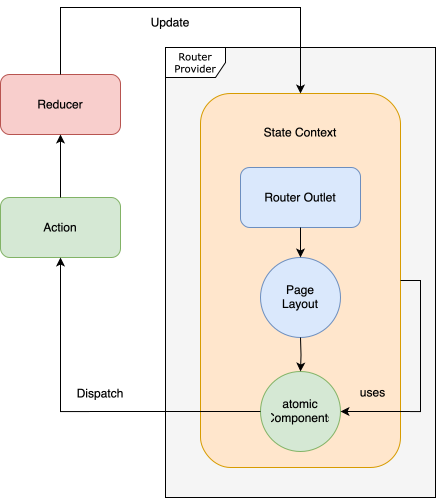
\includegraphics[width=\textwidth]{assets/Flow-Diagram.png}
  \label{fig:flow_chart}
\end{figure}

Pages (rectangles) and Components (circles) that are involved in updating and consuming the state context are presented in Figure  \ref{fig:uml_diagram}.

\begin{figure}[!h]
  \centering
  \caption{Flow of Components involved in updating and consuming the state context}
  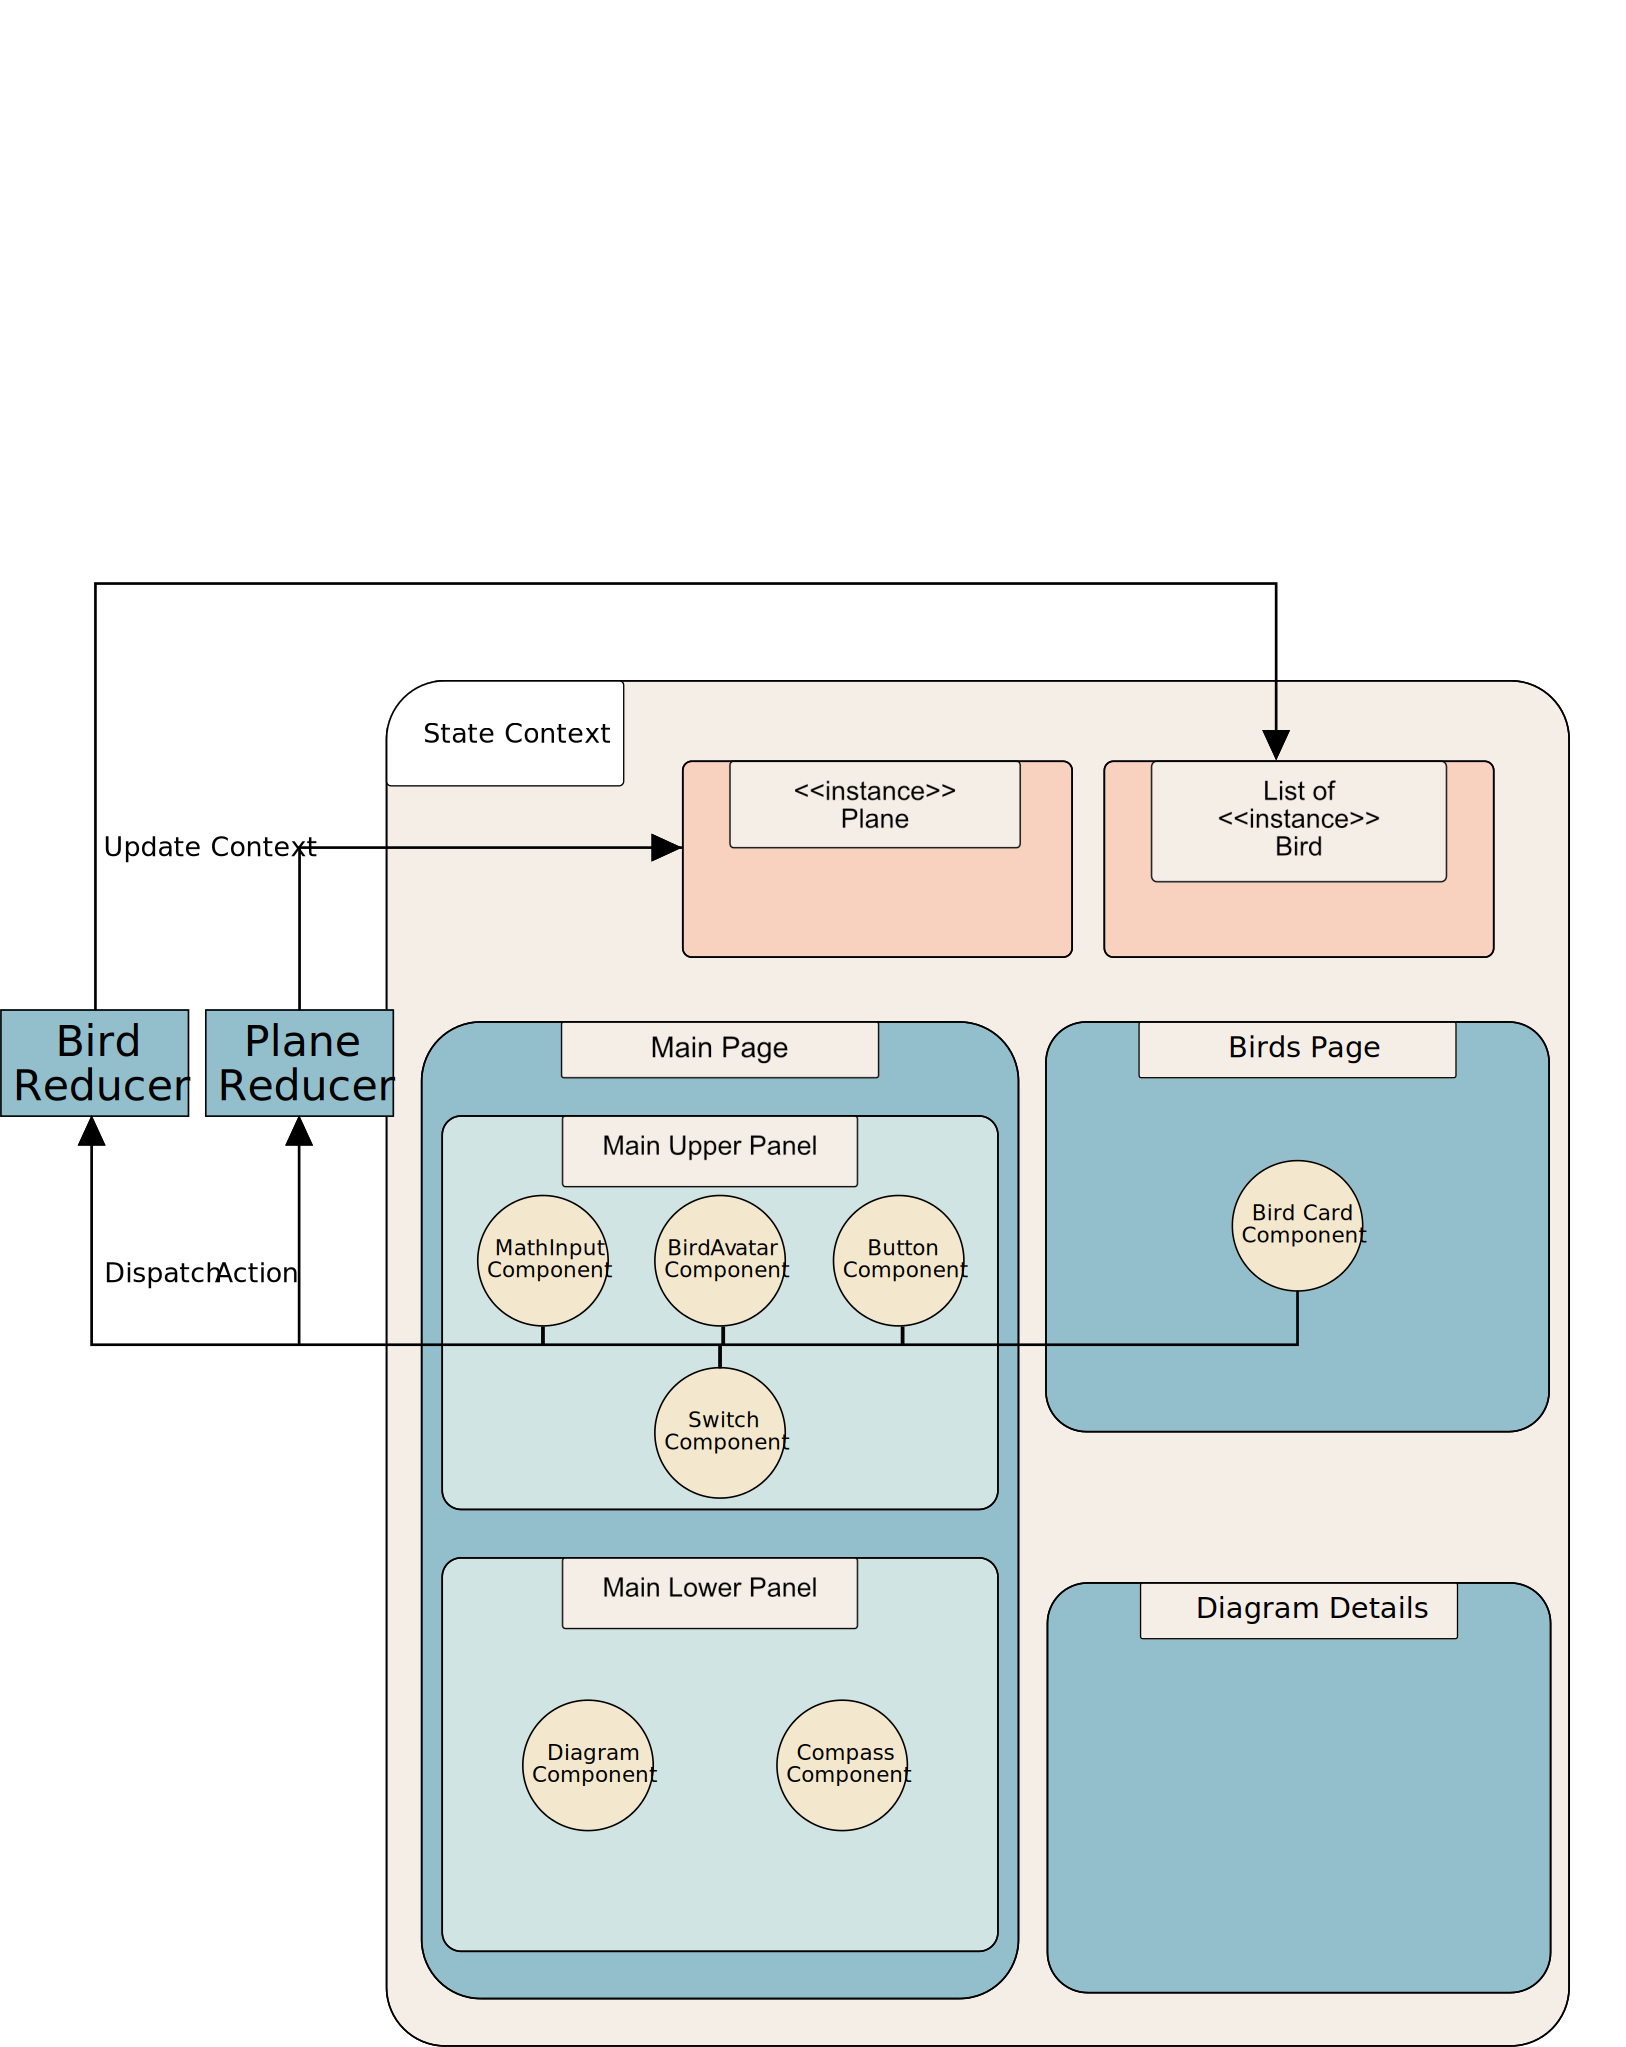
\includegraphics[width=\textwidth]{assets/uml_diagram.png}
  \label{fig:uml_diagram}
\end{figure}

\blankpage
\newpage
\subsection{Design and Implementation Procedure}
The design process was mostly defined by drawing and redefining new mock-ups that were refined after each sprint. The implementation of mathematical functions followed a \ac{TDD} procedure.

\subsection{Used 3rd Party Libraries}
The following 3rd party libraries were finally used in the making of this application.
\begin{itemize}
  \item React (\cite{React}), because of its simple design and vast ecosystem and the "ease" of state updates.
  \item React Router (\cite{ReactRouter}) as a well established way to navigate a website. 
  \item React Icons (\cite{ReactIcons}) as a nice and easy way to display common FontAwesome (\cite{FA}) Icons.
  \item Chakra-UI (\cite{chakra}), again for its ease of use and customizability of existing designs.
  \item PlotlyJS (\cite{PlotlyJS}), because it is the only graphing library I found that I could misuse for drawing shapes rather than the intended purpose of presenting data graphically. On top of it all it is well documented.
  \item Vite (\cite{Vite}) as a modern building tool, to get the app ready for production.
  \item Vitest (\cite{Vitest}), since I'm already using vite, the corresponding testing framework was the only logical choice.
  \item Docker (\cite{Docker}), which was not really necessary for my application in the end. But since the task asked for it, the webserver still runs as a dockerized container, running an NGINX \cite{NGINX} on the backend, serving the distribution version of this web application.
\end{itemize} 
\pagebreak
\section{Test Document}
\subsection{Test Plan}
Test Coverage for all functions that are involved in mathematical calculation shall have 100\% code coverage and shall cover edge cases. Functions and methods involved in mathematical calculations are listed under \enquote{\hyperref[tab:math_functions]{Mathematical Functions}}.

The user interface shall be tested according to the checklist listed under \enquote{\hyperref[tab:manual_tests]{Manual Tests}}. 

\subsection{Manual Tests}
A page reload shall be performed before each test case.

    \bgroup
    \def\arraystretch{1.5}
    \setlength\arrayrulewidth{1.2pt}
    \color{textgray}
    \begin{xltabular}{\textwidth}{|X|X|M{2cm}|M{2cm}|}

\caption*{} \label{tab:manual_tests} \\

\arrayrulecolor{linegray}\hline \rowcolor{lightgray} \multicolumn{1}{|c|}{\color{default}\textbf{Test Case}} & \multicolumn{1}{c|}{\color{default}\textbf{Expected Outcome}} & \multicolumn{1}{c|}{\color{default}\textbf{Satisfies}} & \multicolumn{1}{c|}{\color{default}\textbf{Status}}\\ \hline

 \endfirsthead 
 \multicolumn{4}{c}%
{\tablename\ \thetable{} -- continued from previous page} \\ \hline \multicolumn{1}{|c|}{\textbf{Test Case}} & \multicolumn{1}{c|}{\textbf{Expected Outcome}} & \multicolumn{1}{c|}{\textbf{Satisfies}} & \multicolumn{1}{c|}{\textbf{Status}}\\ \hline 
\endhead \hline 
\multicolumn{4}{|r|}{{Continued on next page}} \\ \hline 
\endfoot

\hline 
 \endlastfoot 
On the \enquote{Paper Plane}-Page, click on \enquote{Add Threat} 6 times. & Only 5 bird avatars shall be displayed and a grey circle showing {\ttfamily\enquote{+1}}. Pay attention that the first bird is the one that disappears after the 5th bird. \newline All birds shall be displayed at {\ttfamily(0,0,0)}. & {\color{purpleT}\ttfamily DLMCSPSE-224 \newline\newline DLMCSPSE-225-1} & \tcbox[colframe=TAGgreen, colback=TAGgreen]{\textbf{\footnotesize PASSED}} \\ \hline 
  Click \enquote{Add bird} without providing any number. \newline Click on the \enquote{X}-Icon next to the birds Avatar. \newline Add a bird at {\ttfamily (101,0,0)}. & A bird shall be added at {\ttfamily (0,0,0)}. \newline Now no bird shall be displayed. \newline No bird shall be added. A toast shall be displayed. & {\color{purpleT}\ttfamily DLMCSPSE-225} & \tcbox[colframe=TAGgreen, colback=TAGgreen]{\textbf{\footnotesize PASSED}} \\ \hline 
  Enter the coordinates {\ttfamily(1,2,3)} and click \enquote{Add Threat}. & A new bird shall be displayed at the specified coordinates. & {\color{purpleT}\ttfamily DLMCSPSE-225-1} & \tcbox[colframe=TAGgreen, colback=TAGgreen]{\textbf{\footnotesize PASSED}} \\ \hline 
  Enter the coordinates {\ttfamily (101,2,3)} and click \enquote{Add Threat}. & No new bird is added and a warning pop-up is displayed. & {\color{purpleT}\ttfamily DLMCSPSE-225-2} & \tcbox[colframe=TAGgreen, colback=TAGgreen]{\textbf{\footnotesize PASSED}} \\ \hline 
  Click \enquote{Add Threat}. Enter the coordinates {\ttfamily (1,2,3)} and click \enquote{Add Threat} again. \newline Click on the little x of the first bird. & Only one bird avatar is displayed at {\ttfamily (1,2,3)} on each page and in the 3D-Scene. & {\color{purpleT}\ttfamily DLMCSPSE-225-3} & \tcbox[colframe=TAGgreen, colback=TAGgreen]{\textbf{\footnotesize PASSED}} \\ \hline 
  Add two birds. \newline Click on a bird.\newline Click on another bird.\newline Click on the same bird again.\newline & First no bird shall be selected. \newline This bird shall now have a ring around it. And the compass component shall display $0$m to <BirdName> and <BirdName> at $0°$. \newline Now the other bird shall have a ring around it and the ring of the first bird shall disappear. \newline Now no bird shall have a ring. The extra values in the compass component shall now dissapear. & {\color{purpleT}\ttfamily DLMCSPSE-226 \newline DLMCSPSE-246} & \tcbox[colframe=TAGgreen, colback=TAGgreen]{\textbf{\footnotesize PASSED}} \\ \hline 
  Move the plane $-3$ on the $x$-axis. & The plane shall not move and a toast shall be displayed. & {\color{purpleT}\ttfamily DLMCSPSE-228-3} & \tcbox[colframe=TAGgreen, colback=TAGgreen]{\textbf{\footnotesize PASSED}} \\ \hline 
  Add a bird at {\ttfamily (50,2,2)} \newline Move the plane $-10$ on the $x$-Axis. & Before doing anything. The scale of the scene shall be {\ttfamily (-6,6)} for $x$/$y$ and {\ttfamily (0,12)} for the $z$-Axis. \newline After the addition of the bird. The scale shall be: {\ttfamily (-50,50)} for $x$/$y$ and {\ttfamily (0,100)} for the $z$-Axis. \newline After the translation the scale shall be {\ttfamily (-60,60)} for $x$/$y$ and {\ttfamily (0,120)} for the $z$-Axis. & {\color{purpleT}\ttfamily DLMCSPSE-229 \newline DLMCSPSE-228-1/2} & \tcbox[colframe=TAGgreen, colback=TAGgreen]{\textbf{\footnotesize PASSED}} \\ \hline 
  Add a bird at {\ttfamily (2,2,-3)}. \newline  Add a bird at {\ttfamily (2,2,2)}. And then try to move the bird z $-3$. \newline And then move the bird x $2$. & No bird shall be added and a toast ist expected. \newline A new dot in the colour of the bird is expected. \newline The bird shall not move and a toast shall pop up. \newline After the second translation the bird shall be at {\ttfamily (4,2,2)}. & {\color{purpleT}\ttfamily DLMCSPSE-232 \newline DLMCSPSE-231} & \tcbox[colframe=TAGgreen, colback=TAGgreen]{\textbf{\footnotesize PASSED}} \\ \hline 
  Rotate the plane yaw $405°$. & The plane shall point NE 45°. & {\color{purpleT}\ttfamily DLMCSPSE-233-2} & \tcbox[colframe=TAGgreen, colback=TAGgreen]{\textbf{\footnotesize PASSED}} \\ \hline 
  Randomly rotate the plane and click on \enquote{reset plane} & the plane shall now be at {\ttfamily 0,0,2}. & {\color{purpleT}\ttfamily DLMCSPSE-235} & \tcbox[colframe=TAGgreen, colback=TAGgreen]{\textbf{\footnotesize PASSED}} \\ \hline 
  Click \enquote{Hide Coordinate System} twice. & After the first click the coordinate system in the scene shall disappear and reappear after the second click. & {\color{purpleT}\ttfamily DLMCSPSE-239} & \tcbox[colframe=TAGgreen, colback=TAGgreen]{\textbf{\footnotesize PASSED}} \\ \hline 
  Add a bird at {\ttfamily (2,2,2)}. And navigate to the \enquote{Bird} Page. \newline Navigate back. & A bird card shall be visible displaying the following information: \newline $2.83$ Meter \newline $2.83$ Meter \newline $-0.73$ Degree \newline $3.13$ Meter \newline After navigating back the information shall not be lost. & {\color{purpleT}\ttfamily DLMCSPSE-240} & \tcbox[colframe=TAGgreen, colback=TAGgreen]{\textbf{\footnotesize PASSED}} \\ \hline 
  Add a bird at {\ttfamily(3.3,0,0)}. \newline move to the \enquote{Birds} component and check. \newline move back and translate the bird {\ttfamily(0,0,3.3)} and move back to the Bird Cards. \newline & The point {\ttfamily(0,0,3.3)} is the planes marble. So an elevation angle of $-45°$ is to be expected. \newline After translation an angle of $0°$ is expected. & {\color{purpleT}\ttfamily DLMCSPSE-240-f} & \tcbox[colframe=TAGgreen, colback=TAGgreen]{\textbf{\footnotesize PASSED}} \\ \hline 
  Rotate the plane yaw $90°$. \newline Add another rotation yaw $225°$. & Before doing anything, the plane in the compass component shall point north. \newline After the rotation the plane shall point East. After the second rotation the plane shall point NW ($-45°$) & {\color{purpleT}\ttfamily DLMCSPSE-244} & \tcbox[colframe=TAGgreen, colback=TAGgreen]{\textbf{\footnotesize PASSED}} \\ \hline 
  Add a Threat at (2,2,2). & A Bird Icon shall be displayed at roughly $315°$/$-45°$ in the compass component. & {\color{purpleT}\ttfamily DLMCSPSE-245-1} & \tcbox[colframe=TAGgreen, colback=TAGgreen]{\textbf{\footnotesize PASSED}} \\ \hline 
  Add a Threat at {\ttfamily (14,0,0)} and a Threat at {\ttfamily (13,0,0)}. & The first one shall be indicated by an arrow and the second one shall be indicated by an icon at $0°$ & {\color{purpleT}\ttfamily DLMCSPSE-245-2} & \tcbox[colframe=TAGgreen, colback=TAGgreen]{\textbf{\footnotesize PASSED}} \\ \hline 
  
\end{xltabular} 
 \egroup 
 \color{default}

\newpage
\subsection{Mathematical Functions}

List of functions and methods that are involved in mathematical calculations and are therefore essential to test properly. Coverage is calculated by the {\ttfamily vitest} testing framework.

    \bgroup
    \def\arraystretch{1.5}
    \setlength\arrayrulewidth{1.2pt}
    \color{textgray}
    \begin{xltabular}{\textwidth}{|M{1.2cm}|X|X|M{3cm}|}

\caption*{} \label{tab:Requirements - Functional} \\

\arrayrulecolor{linegray}\hline \rowcolor{lightgray} \multicolumn{1}{|c|}{\color{default}\textbf{ID}} & \multicolumn{1}{c|}{\color{default}\textbf{Function/Method}} & \multicolumn{1}{c|}{\color{default}\textbf{Description}} & \multicolumn{1}{c|}{\color{default}\textbf{Coverage}}\\ \hline

 \endfirsthead 
 \multicolumn{4}{c}%
{\tablename\ \thetable{} -- continued from previous page} \\ \hline \multicolumn{1}{|c|}{\textbf{ID}} & \multicolumn{1}{c|}{\textbf{Function/Method}} & \multicolumn{1}{c|}{\textbf{Description}} & \multicolumn{1}{c|}{\textbf{Coverage}}\\ \hline 
\endhead \hline 
\multicolumn{4}{|r|}{{Continued on next page}} \\ \hline 
\endfoot

\hline 
 \endlastfoot 
\textbf{ F1 } & {\ttfamily azimuthAngle(A: Point, center?: Point): number} & Calculates the angle measure (in radians, with $-\pi \textless \theta \le \pi$ between the positive x-axis and the ray from the origin to the point {\ttfamily(x,y)} in the Cartesian plane.\newline If a center point is provided, the angle is calculated from the new center position. & \tcbox[colframe=TAGgreen, colback=TAGgreen]{\textbf{\footnotesize 100\%}} \\ \hline 
  
\end{xltabular} 
 \egroup 
 \color{default}
    
\newpage
\subsection{Automated Tests}
A list of test cases that cover all math functions and the requirements they are testing.

    \bgroup
    \def\arraystretch{1.5}
    \setlength\arrayrulewidth{1.2pt}
    \color{textgray}
    \begin{xltabular}{\textwidth}{|M{1.2cm}|M{1.2cm}|X|M{1.8cm}|M{3cm}|}

\caption*{} \label{tab:Requirements - Functional} \\

\arrayrulecolor{linegray}\hline \rowcolor{lightgray} \multicolumn{1}{|c|}{\color{default}\textbf{Test ID}} & \multicolumn{1}{c|}{\color{default}\textbf{ID}} & \multicolumn{1}{c|}{\color{default}\textbf{Test}} & \multicolumn{1}{c|}{\color{default}\textbf{Satisfies}} & \multicolumn{1}{c|}{\color{default}\textbf{Status}}\\ \hline

 \endfirsthead 
 \multicolumn{5}{c}%
{\tablename\ \thetable{} -- continued from previous page} \\ \hline \multicolumn{1}{|c|}{\textbf{Test ID}} & \multicolumn{1}{c|}{\textbf{ID}} & \multicolumn{1}{c|}{\textbf{Test}} & \multicolumn{1}{c|}{\textbf{Satisfies}} & \multicolumn{1}{c|}{\textbf{Status}}\\ \hline 
\endhead \hline 
\multicolumn{5}{|r|}{{Continued on next page}} \\ \hline 
\endfoot

\hline 
 \endlastfoot 
T1 & F1 & Calc angle from center (7,7) to the points: (7,3), (20,7), (7,10), (3,7), (6.9, 3) and (7.1, 3) & {\color{purpleT}\ttfamily TECH-001} & \tcbox[colframe=TAGgreen, colback=TAGgreen]{\textbf{\footnotesize PASSED}} \\ \hline 
  
\end{xltabular} 
 \egroup 
 \color{default} 
\pagebreak
\section{Finalisation Phase}
\subsection{Sprint Retrospective - Main Take-Aways}
Especially when working alone, complacency of procedure becomes a major issue and needs to get extra attention during future projects.

It is vital for future project plans and/or deadlines to be more realistic in terms of what is achievable in the given time/cost-frame.

\subsection{Methodologies and Tool}
You should especially reflect on the applied tools, methodologies, and techniques and on your handling of the resources 
\pagebreak
\section{Glossary}
\input{chapters/X_Glossary} 
\pagebreak
%% ++++++++++++++++++++++++++++++++++++++++++
%% Literatur
%% ++++++++++++++++++++++++++++++++++++++++++
\blankpage

\phantomsection
% set bibliography name
\renewcommand{\bibname}{Literaturverzeichnis}
\addcontentsline{toc}{section}{\bibname}
% \nocite{*} % nur angeben, wenn auch nicht im Text zitierte Quellen 

\begin{flushleft}

\printbibliography[title=\bibname]
\end{flushleft}

% %% ++++++++++++++++++++++++++++++++++++++++++
% %% Anhang
% %% ++++++++++++++++++++++++++++++++++++++++++
% \blankpage
% \appendix
% \include{pages/appendix} % Anhang % TODO: Add Appendix?

\end{document}

